%!TEX root = /Users/jakubkonka/Thesis/Thesis.tex
\chapter{Casting Network Selection Mechanism into Common Priors Setting}
\label{cha:approximation}

\minitoc
\vspace{10mm}

This chapter explores whether an auction format represented by the DMP selling mechanism can be modeled as an asymmetric first-price sealed-bid auction (FPA) with common priors; that is, an auction in which bidders are characterised by different probability distributions sharing a common support. Ideally, if the DMP auction was shown to be a special case of some corresponding common priors auction, then the numerical solution methods presented in Hubbard and Parsch~\cite{HubbardPaarsch2011}, and extensively studied by the economic community, could be employed. Conversely, if the DMP auction format cannot be shown to constitute a special case of the common priors auction, then, provided the expected profits for the bidders in both auction formats differ only slightly, the common priors auction could still effectively be used to approximate the solution to the DMP auction.

\section{Mathematical Description} % (fold)
\label{sec:mathematical_description_approximation}

Following the notation of Chapter~\ref{cha:indirect}, let each bidder $i$ be characterised by the utility function
\begin{equation}
  \label{eq:utility_approximation}
    u_i(b,c) = \left\{
  \begin{array}{l l}
    b_i-c_i & \;\text{if } b_i < \displaystyle\min_{j\neq i}b_j,\\
    0 & \;\text{if } b_i > \displaystyle\min_{j\neq i}b_j,
  \end{array}\right.
\end{equation}
where, as before, $b = (b_1,\ldots,b_n)$, and $c = (c_1,\ldots,c_n)$. In the common priors auction, we assume that each bidder $i$ draws their cost from common support across all bidders; i.e., let
\begin{equation*}
  c_i\in [\underline{c}, \bar{c}] \quad\text{for all } i\in N \text{ such that } [\underline{c}, \bar{c}]\subseteq [0, 1].
\end{equation*}

Let $F_i$ be the distribution function of $c_i$ for all $i\in N$. Note that the distribution functions between bidders need not be equal, and hence, we are dealing with an asymmetric FPA.

We further assume that
\begin{assumptions}
\label{ass:assumptions_common_priors_approximation}
Assume that
\begin{enumerate}
  \item $F_i$ is differentiable over $(\underline{c}, \bar{c}]$ with a derivative $f_i$ locally bounded away from zero over this interval;
  \item $F_i$ is atomless; and
  \item $F_i(c)>0$ for all $c\in [\underline{c}, \bar{c}]$ and $i\in N$.
\end{enumerate}
\end{assumptions}
These assumptions correspond to Assumptions~A.1 and Theorem~U.1 in Lebrun~\cite{Lebrun2006}, and, as shown by Lebrun, with these assumptions satisfied, there exists one and only one pure-strategy Bayesian Nash equilibrium where bidders engage in serious bidding; that is, bid at least their cost. Formally,
\begin{proposition}[Characterization of the Equilibrium in Common Priors Setting]
\label{prop:characterization_of_the_equilibrium_in_common_priors_setting_approximation}
Let Assumptions~\ref{ass:assumptions_common_priors_approximation} be satisfied. There exists one and only one pure-strategy Bayesian Nash equilibrium where bidders submit at least their costs. In every such equilibrium, bidder $i\in N$ follows a bid function $b_i$, for all $1\leq i\leq n$ such that its inverse, $c_i\equiv b_i^{-1}$, satisfy the following system of differential equations
\begin{equation*}
  \frac{d}{db}c_i(b) = \frac{1 - F_i(c_i(b))}{f_i(c_i(b))}\left[ \frac{1}{n-1}\sum_{k=1}^n \frac{1}{b-c_k(b)} - \frac{1}{b-c_i(b)} \right]
\end{equation*}
for all $1\leq i\leq n$, with the following lower boundary condition
\begin{equation}
  \label{eq:foc_ode_lower_boundary_approximation}
  c_i(\underline{b}) = \underline{c}
\end{equation}
and the upper boundary condition
\begin{equation}
  \label{eq:foc_ode_upper_boundary_approximation}
  c_i(\bar{c}) = \bar{c}
\end{equation}
for all $1\leq i\leq n$.
\end{proposition}
\noindent The formal proof of Proposition~\ref{prop:characterization_of_the_equilibrium_in_common_priors_setting_approximation} as well as any other proposition (unless stated otherwise) included in this chapter is given in Section~\ref{sec:proofs_approximation}.

In effect, Proposition~\ref{prop:characterization_of_the_equilibrium_in_common_priors_setting_approximation} is a special case of Proposition~\ref{prop:characterization_of_the_equilibrium_indirect}. That is, the equilibrium bidding functions still have to satisfy the system of nonlinear ODEs given by Equation~\eqref{eq:foc_ode_indirect}; however, in this case, the lower boundary condition reduces to
\begin{equation*}
  c_i(\underline{b}) = \underline{c},
\end{equation*}
and the upper boundary condition to
\begin{equation*}
  c_i(\bar{c}) = \bar{c},
\end{equation*}
i.e., the bids never exceed the upper extremity of the common support range.

It should be noted that, even though the bidding problem is considerably simpler than the original one discussed in this thesis (cf.~Chapter~\ref{cha:indirect}), it still involves finding the lower bound on bids, and hence, the closed-form solution exists only in a handful of special cases~\cite{Krishna10,HubbardPaarsch2011}.

% section mathematical_description (end)

\section{Numerical Solutions} % (fold)
\label{sec:numerical_solutions}

As already mentioned in the previous chapter, however, the problem can be approximated using numerical methods (see Hubbard and Paarsch~\cite{HubbardPaarsch2011} for an excellent discussion). In this chapter, a common priors auction is approximated using the forward shooting method (FSM), but tailored to the problem at hand. The FSM method was chosen due to its relatively low implementation complexity, and the fact that a similar method was used to solve the DMP bidding problem. Therefore, the numerical solutions to the DMP and common priors auctions should be of comparable quality (in terms of the numerical accuracy and stability).

\subsection{Forward Shooting Method} % (fold)
\label{sub:forward_shooting_method}

To briefly recap, the FSM method was first proposed by Bajari~\cite{Bajari2001a} (cf.~Algorithm~1 in \cite{Bajari2001a}). The method aims at finding the best approximation of the lower bound on bids, $\underline{b}$, by successively picking a value from the feasible interval, $(\underline{c}, \bar{c})$, and verifying whether a numerical solution to the initial value problem
\begin{equation}
  \label{eq:fsm_initial_value_problem_approximation}
  \begin{array}{ll}
     \displaystyle\frac{d}{db}c_i(b) &= \displaystyle\frac{1 - F_i(c_i(b))}{f_i(c_i(b))}\left[ \frac{1}{n-1}\sum_{k=1}^n \frac{1}{b-c_k(b)} - \frac{1}{b-c_i(b)} \right]\\[2ex]
    c_i(\underline{b}) &= \underline{c}
  \end{array}
\end{equation}
for all $i\in N$, lies within a set of permissible functions, $S$, such that every element of that set is a function mapping $[\underline{b}, \bar{c}]$ into $[\underline{c}, \bar{c}]$, it is monotonically increasing everywhere except possibly at $\underline{c}$, and each function value is strictly lower than its argument except possibly at $\bar{c}$; that is,
\begin{equation*}
  S\equiv\left\{s \:\middle\vert\:
  \begin{array}{l}
    s: [\underline{b}, \bar{c}]\to [\underline{c}, \bar{c}],\\
    b_1 < b_2\implies s(b_1) < s(b_2) \text{ for all }b_1,b_2\in [\underline{b}, \bar{c}),\\
    s(b) < b \text{ for all }b\in [\underline{b}, \bar{c})
  \end{array}
  \right\}.
\end{equation*}

The pseudo-code for the FSM is depicted in listing Algorithm~\ref{alg:forward_shooting_method_approximation}. Note that the algorithm is almost identical to the FSM version tailored to the DMP auction (cf.~Algorithm~\ref{alg:forward_shooting_method_indirect}), with only differences being the definition of the set of permissible functions, $S$, and the algorithm's search region delimited by $low$ and $high$ variables. Hence, we omit the discussion of the algorithm and refer the Reader to Section~\ref{sub:forward_shooting_method_indirect}.

\begin{algorithm}
\caption{Forward shooting method (common priors version)}
\label{alg:forward_shooting_method_approximation}
\begin{algorithmic}[1]
\Require{$\epsilon\in (0, \bar{c} - \underline{c}); low, high\in [\underline{c}, \bar{c}]$ such that $low\leq high$}
\Ensure{Approximation to $\underline{b}$}
  \Statex
  \Let{$low$}{$\underline{c}$}
  \Let{$high$}{$\bar{c}$}
  \Statex
  \While{$high-low > \epsilon$}
    \Let{$guess$}{$0.5\cdot(low + high)$}
    \Let{$bids$}{$[guess, \bar{c})$}
    \Let{$(costs_1,\dotsc,costs_n)$}{solve~\eqref{eq:fsm_initial_value_problem_approximation} with initial value $\underline{b} = guess$}
    \StatexIndent[7.5]{evaluated at points $b\in bids$}
    \If{$(bids,costs_i)\in S$ for all $i\gets 1$ to $n$}
      \Let{$high$}{$guess$}
    \Else
      \Let{$low$}{$guess$}
    \EndIf
  \EndWhile
  \Statex
  \Let{$\underline{b}$}{$0.5\cdot(low + high)$}
\end{algorithmic}
\end{algorithm}

Similarly to the implementation of the FSM algorithm for the DMP auction, the approximation results presented in this chapter have been derived using the GNU Scientific Library (GSL) implementation of the Embedded Runge-Kutta-Fehlberg (4,5) method.

% subsection forward_shooting_method (end)

\subsection{Verification} % (fold)
\label{sub:verification}

Before proceeding with the modelling and analysis, the FSM algorithm was tested for correct implementation. The bidding scenario used to verify the algorithm is taken from the Bajari's paper \cite{Bajari2001a}. There are three bidders, and each is characterised by a truncated normal distribution but with different mean and standard deviation parameters (Table~\ref{tab:verification_approximation}). Furthermore, each bidder draws their cost from common range of costs, $c_i\in [2,8]$.

\begin{table}[t]
  \caption{Test bidding scenario}
  \vspace{0.5cm}
  \begin{tabular*}{0.5\columnwidth}[L]{@{\extracolsep{\fill}}r c c}
    \hlx{vhv}
    & \textbf{Mean}, $\mu_i$ & \textbf{Standard deviation}, $\sigma_i$\\
    \hlx{vhv}
    \textbf{Bidder 1} & $4$ & $1.5$\\
    \textbf{Bidder 2} & $5$ & $1.5$\\
    \textbf{Bidder 3} & $6$ & $1.5$\\
    \hlx{vhs}
  \end{tabular*}
  \label{tab:verification_approximation}
\end{table}

Figure~\ref{fig:fsm_common_priors_verification_approximation} depicts the numerically approximated solution to the problem. It is clear that the approximation agrees with that of Bajari's~\cite{Bajari2001a} (cf.~Figure~1 in \cite{Bajari2001a}). Furthermore, in Figure~\ref{fig:fsm_common_priors_verification_sufficiency_approximation}, the numerical solution is verified whether it satisfies the sufficiency condition for an equilibrium; that is, whether the numerically derived bidding strategy for each bidder is a best response to the bidding strategies of the remaining bidders. As expected, the solution satisfies the sufficiency condition, and hence, we conclude that the algorithm was implemented correctly.

\begin{figure}[p!]
  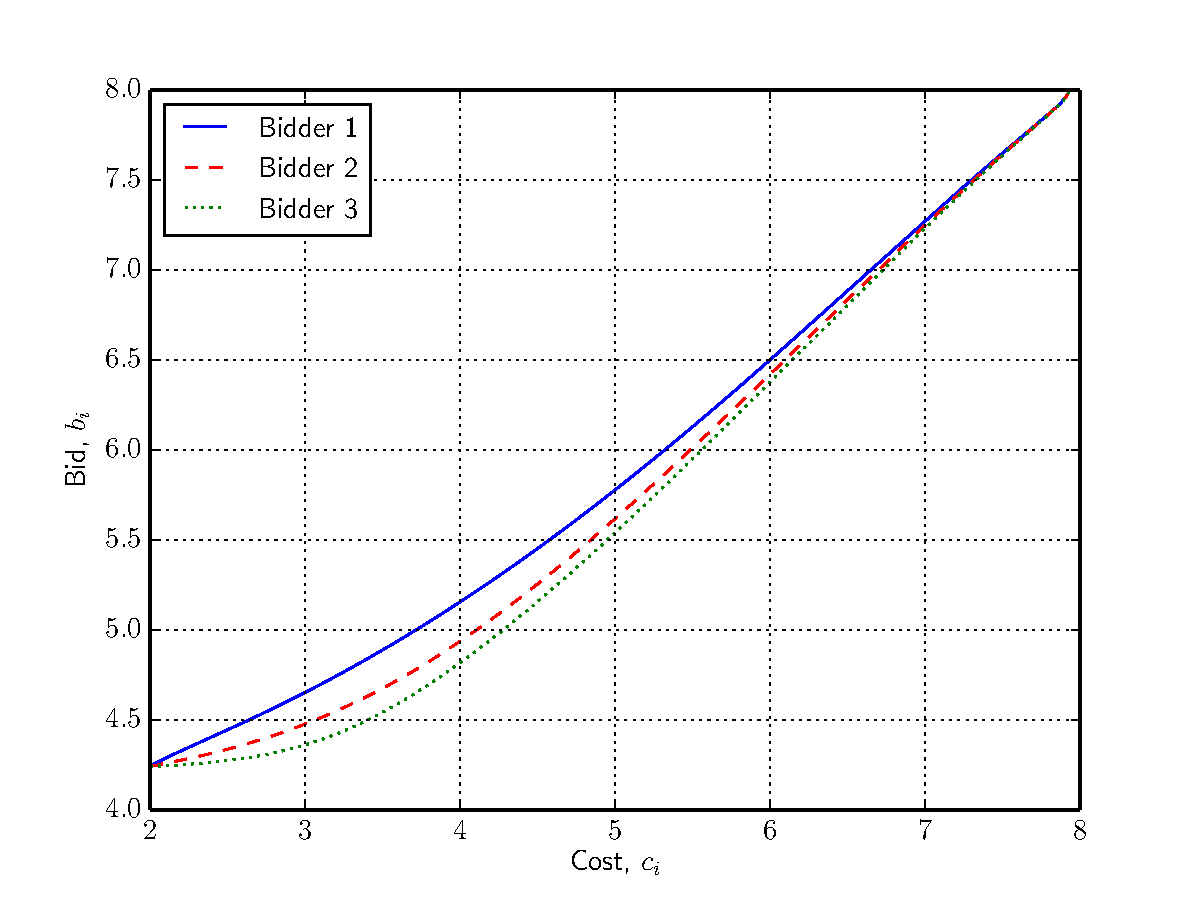
\includegraphics[width=\figsize]{Approximation/Figures/fsm_common_priors_verification}
  \caption{FIX:ME FSM Common Priors verification}
  \label{fig:fsm_common_priors_verification_approximation}
  \vspace{10mm}
  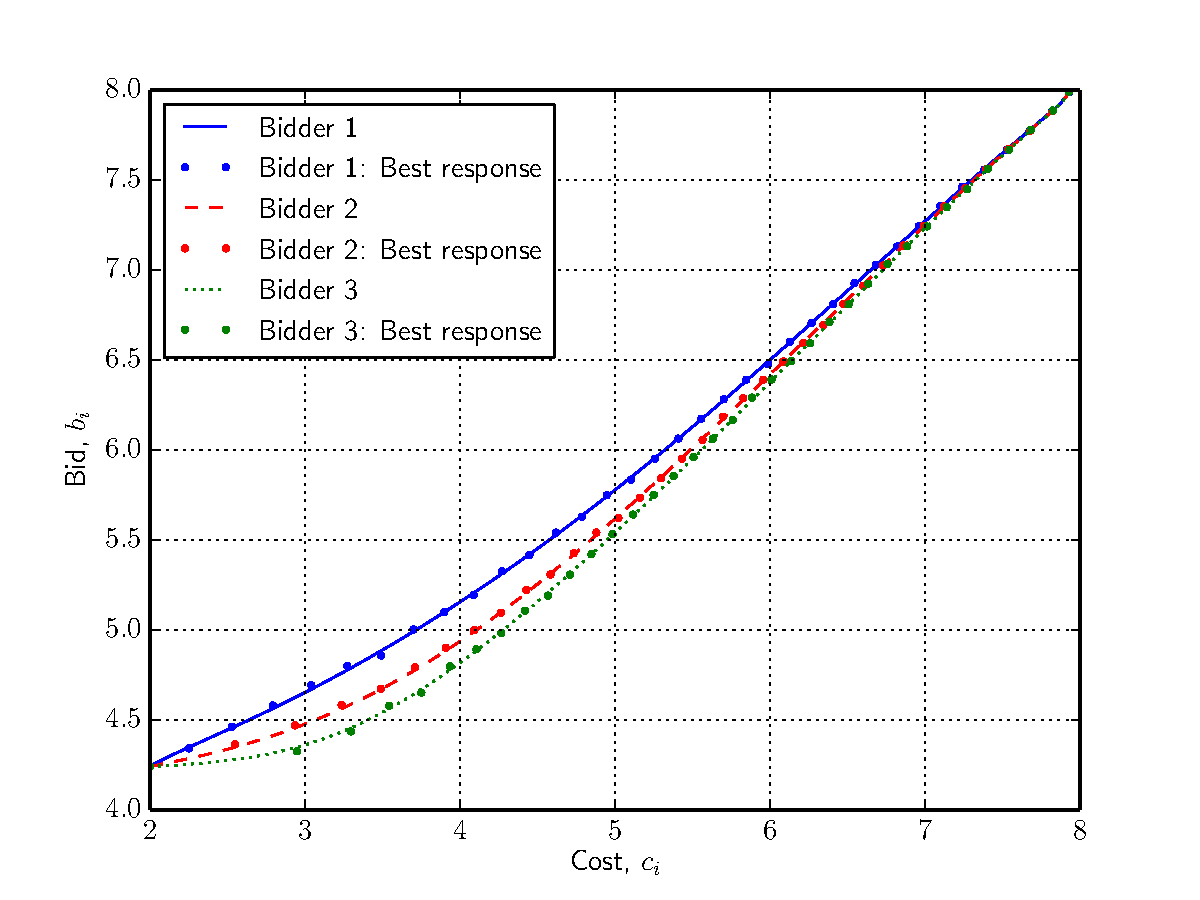
\includegraphics[width=\figsize]{Approximation/Figures/fsm_common_priors_verification_sufficiency}
  \caption{FIX:ME FSM Common Priors verification}
  \label{fig:fsm_common_priors_verification_sufficiency_approximation}
\end{figure}

% subsection verification (end)

% section numerical_solutions (end)

\section{Network Selection Mechanism Cast into Common Priors Setting} % (fold)
\label{sec:network_selection_mechanism_cast_into_common_priors_setting_approximation}
In this section, we discuss the results of approximating the DMP auction with a common priors (CP) auction. To this end, we firstly model the DMP auction as a CP auction where bidders are characterised by costs distributed according to a truncated normal distribution. Then, the methodology used to quantify the accuracy of approximations is outlined. Lastly, the results of approximation for different bidding scenarios ($n\geq 2$ bidders, varying price weight, $w$, and reputations, $r_i$ for all $i\in N$, etc.) are presented and discussed.

\begin{figure}[p!]
  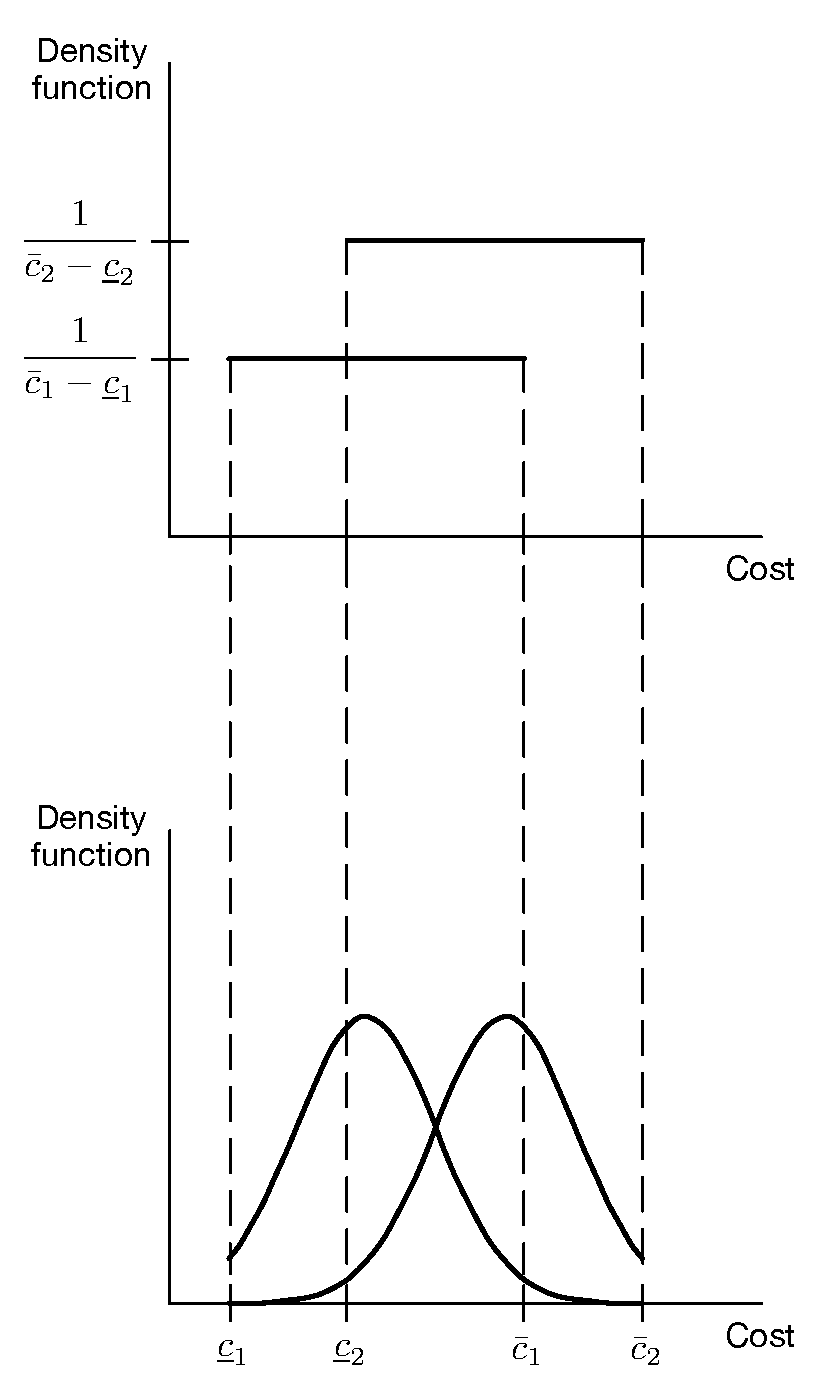
\includegraphics[width=\figsize]{Approximation/Figures/dmp_to_common_priors}
  \caption{FIX:ME DMP auction cast to CP auction}
  \label{fig:dmp_to_common_priors_approximation}
\end{figure}

\subsection{Modelling using Truncated Normal Distribution} % (fold)
\label{sub:modeling_using_truncated_normal_distribution_approximation}
Recall from Chapter~\ref{cha:indirect} that, in the DMP auction, each bidder $i$ draws their cost\footnote{In order to ease the exposition of the concepts presented in this chapter, we shall refer to costs-hat, $\hat{c}_i$, introduced in Chapter~\ref{cha:indirect} as simply costs, $c_i$.} from a uniform distribution with the support
\begin{equation*}
  [(1-w)r_i, (1-w)r_i + w] = [\underline{c}_i, \bar{c}_i] \subset [0,1]
\end{equation*}
Therefore, in the general case, unless the bidders are characterised by the same reputation rating, that is $r_i=r_j$ for all $i,j\in N$, their distributions' supports will not overlap fully; i.e.,
\begin{equation*}
  [\underline{c}_i,\bar{c}_i] \neq [\underline{c}_j,\bar{c}_j], \quad i\neq j \text{ and } i,j\in N.
\end{equation*}

Recall further that, in a CP auction, every bidder is characterised by a distribution (of costs) with common support across all bidders. Hence, in order to model any DMP bidding scenario, firstly, we need to agree on a support that is common to every bidder and, at the same time, encompasses the supports of every individual bidder from the original (DMP) auction. The smallest such support\footnote{To see this, recall that, for any given $w\in (0,1)$, assuming $r_1\leq\cdots\leq r_n$ with at least one inequality strict, it follows $\underline{c}_1\leq\cdots\leq\underline{c}_n$ and $\bar{c}_1\leq\cdots\leq\bar{c}_n$ with at least one inequality strict. If we further let $C_i = [\underline{c}_i, \bar{c}_i]$ then $C = \bigcup_{i\in N} C_i$ is the smallest set containing all sets $C_i$ for all $i\in N$. Since $C_i$ is closed for all $i\in N$, it follows that $C$ is closed, and $C = [\underline{c}, \bar{c}]$ such that $\underline{c} \leq \underline{c}_i$ and $\bar{c}_i\leq \bar{c}$ for all $i\in N$, which is equivalent to $[\min_{i\in N}\{\underline{c}_i\}, \max_{i\in N}\{\bar{c}_i\}]$.} is
\begin{equation}
  \label{eq:domain_common_priors_approximation}
  \displaystyle\left[\min_{i\in N}\{\underline{c}_i\}, \max_{i\in N}\{\bar{c}_i\}\right] \subset [0,1].
\end{equation}
All that remains is to then select a family of distributions which captures the numerical ranges of the original supports as closely as possible.

To provide an illustrative example, let there be 2 bidders such that $\underline{c}_1 < \underline{c}_2 < \bar{c}_1 < \bar{c}_2$. Each bidder is characterised by a uniform distribution, $\mathcal{U}_i$. One possible way of casting this scenario into common priors setting is to model the distributions of both bidders as truncated normal distributions, $\mathcal{N}_i$, truncated to the interval $[\underline{c}_1, \bar{c}_2]$, and with differing mean and standard deviation parameters. This is depicted in Figure~\ref{fig:dmp_to_common_priors_approximation}.

In order to describe the truncated normal distribution, firstly recall the probability density function (pdf) of standard normal distribution
\begin{equation}
  \label{eq:pdf_standard_normal_approximation}
  \displaystyle\phi(x) = \frac{1}{\sqrt{2\pi}} \exp\left\{-\frac{1}{2}x^2\right\},
\end{equation}
and cumulative distribution function (cdf)
\begin{equation}
  \label{eq:cdf_standard_normal_approximation}
  \displaystyle\Phi(x) = \int_{-\infty}^{x}\phi(x)dx = \frac{1}{2}\left[ 1 + \erf\left(\frac{x}{\sqrt{2}}\right) \right]
\end{equation}
for all $x\in\mathbb{R}$. The pdf of the truncated normal distribution, truncated to the interval $x\in[a,b]$, can then be described in terms of the pdf of the standard normal distribution as follows
\begin{equation}
  \label{eq:pdf_truncated_normal_approximation}
  \displaystyle f(x; \mu, \sigma, a, b) = \frac{\frac{1}{\sigma}\phi\left(\frac{x-\mu}{\sigma}\right)}{\Phi\left(\frac{b-\mu}{\sigma}\right) - \Phi\left(\frac{a-\mu}{\sigma}\right)}
\end{equation}
where $\mu\in\mathbb{R}$ is the mean (or location) of the distribution, and $\sigma^2\geq 0$ is the variance (or squared scale)~\cite{JohnsonNormal1994,Cohen1991}. Similarly, the cdf of the truncated normal distribution can be defined as follows
\begin{equation}
  \label{eq:cdf_truncated_normal_approximation}
  \displaystyle F(x; \mu, \sigma, a, b) = \int_{-\infty}^{x}f(x;\mu,\sigma,a,b)dx
  = \frac{\Phi\left(\frac{x-\mu}{\sigma}\right) - \Phi\left(\frac{a-\mu}{\sigma}\right)}{\Phi\left(\frac{b-\mu}{\sigma}\right) - \Phi\left(\frac{a-\mu}{\sigma}\right)}.
\end{equation}

Before moving on to discussing the methodology for quantifying the accuracy of the approximations, consider bidding scenario summarized in Table~\ref{tab:verification_indirect} in Chapter~\ref{cha:indirect}. Suppose we were to cast this scenario into common priors setting where bidders are characterised by truncated normal distributions. Firstly, we note that the supports for both bidders are
\begin{equation*}
  [\underline{c}_1, \bar{c}_1] = [0.125, 0.625]
\end{equation*}
for bidder 1, and
\begin{equation*}
  [\underline{c}_2, \bar{c}_2] = [0.375, 0.875]
\end{equation*}
for bidder 2, while the common support is given by
\begin{equation*}
  [\underline{c}_1, \bar{c}_2] = [0.125, 0.875].
\end{equation*}

\begin{figure}[t]
  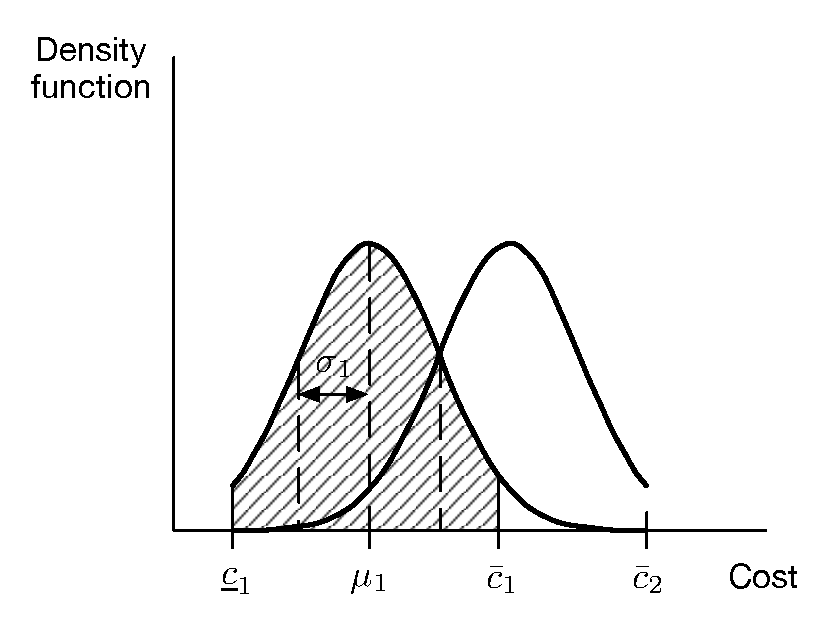
\includegraphics[width=\figsize]{Approximation/Figures/modelling_params}
  \caption{FIX:ME}
  \label{fig:modelling_params_approximation}
\end{figure}

Secondly, we need to specify distribution specific parameters (mean and standard deviation) for each bidder. Since the aim is to approximate the original distributions of both bidders, we pick the midpoints of the original supports as means for both bidders, that is,
\begin{equation*}
  \mu_i = \underline{c}_i + \frac{\bar{c}_i - \underline{c}_i}{2} = \underline{c}_i + \frac{w}{2},
\end{equation*}
and let the standard deviations be equal to the quarter of the length of the original supports, that is,
\begin{equation*}
  \sigma_i = \frac{\bar{c}_i - \underline{c}_i}{4} = \frac{w}{4}.
\end{equation*}
The choice of the parameters is motivated by the shape of the normal distribution~\cite{JohnsonNormal1994}, and the fact that, with this choice of parameters, the probability of at least $0.95$ of drawing cost from the interval $[\underline{c}_i, \bar{c}_i]$ (which corresponds to the interval $[\mu_i - 2\sigma_i, \mu_i + 2\sigma_i]$) is achieved; and therefore, minimising the probability of drawing cost from outside the interval $[\underline{c}_i, \bar{c}_i]$, and effectively imitating uniform distribution with support $[\underline{c}_i, \bar{c}_i]$. This is depicted in Figure~\ref{fig:modelling_params_approximation} as a shaded region under the bell curve.

\begin{table}[b]
  \caption{FIX:ME}
  \vspace{0.5cm}
  \begin{tabular*}{0.5\columnwidth}[L]{@{\extracolsep{\fill}}r c c}
    \hlx{vhv}
    & \textbf{Mean}, $\mu_i$ & \textbf{Standard deviation}, $\sigma_i$\\
    \hlx{vhv}
    \textbf{Bidder 1} & $0.375$ & $0.125$\\
    \textbf{Bidder 2} & $0.625$ & $0.125$\\
    \hlx{vhs}
  \end{tabular*}
  \label{tab:test_truncated_normal_params_approximation}
\end{table}

\begin{figure}[p!]
  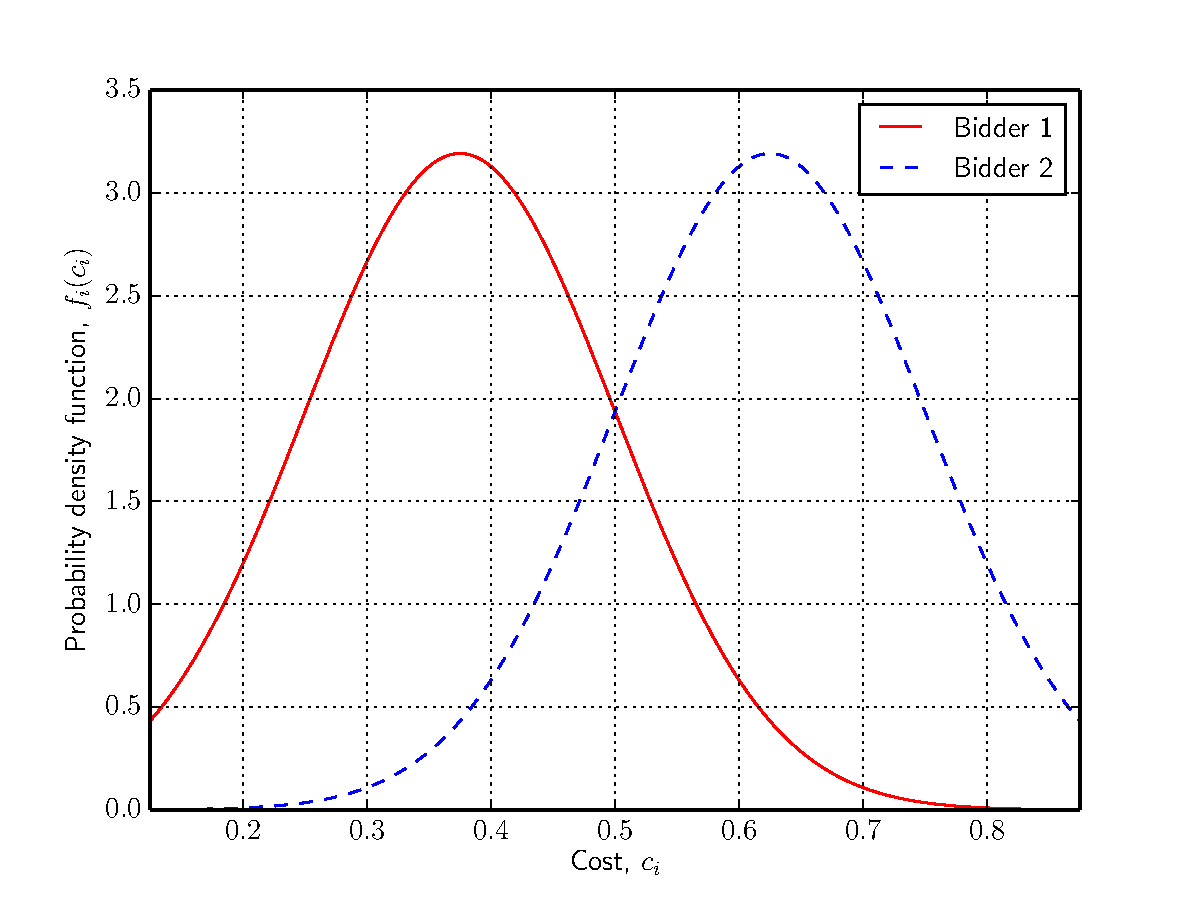
\includegraphics[width=\figsize]{Approximation/Figures/test_truncated_normal_pdfs}
  \caption{FIX:ME}
  \label{fig:test_truncated_normal_pdfs_approximation}
  \vspace{10mm}
  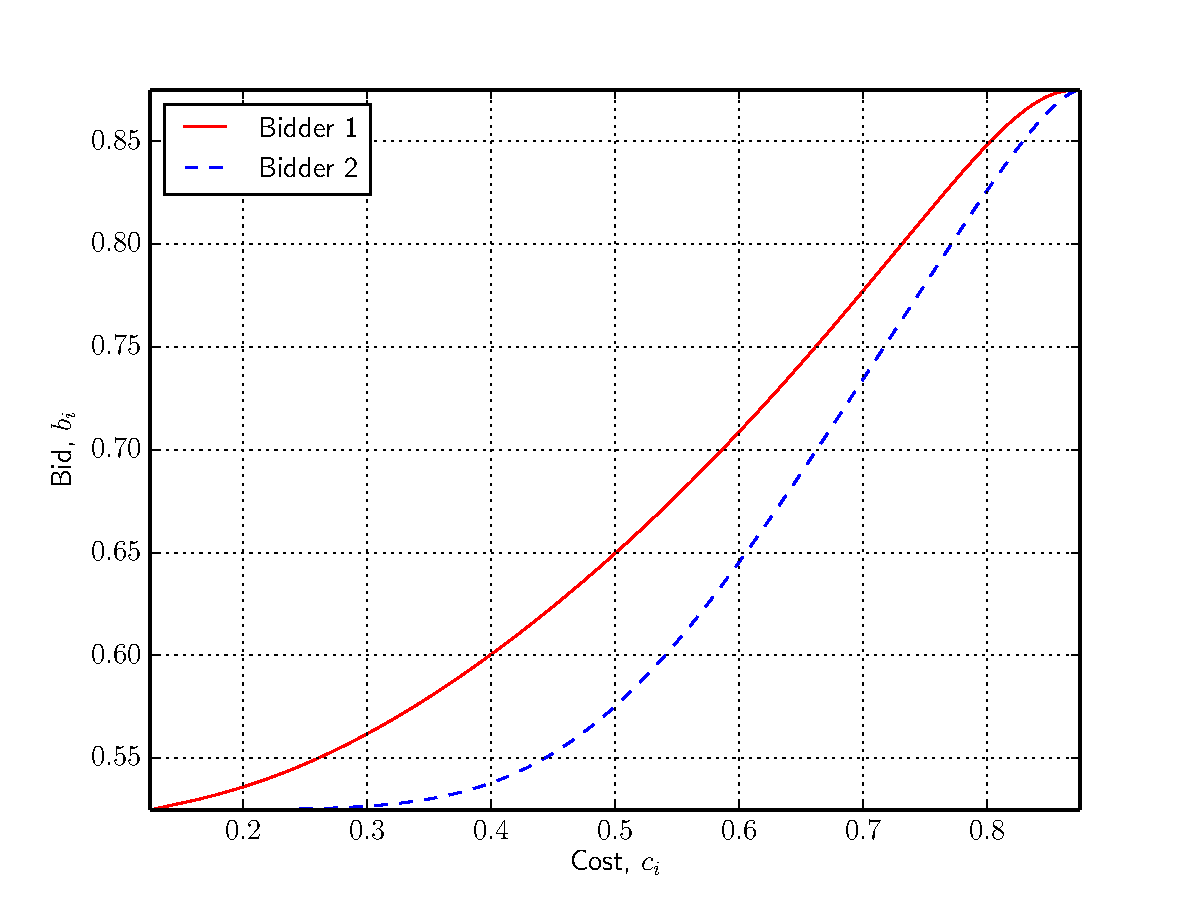
\includegraphics[width=\figsize]{Approximation/Figures/test_truncated_normal_bids}
  \caption{FIX:ME}
  \label{fig:test_truncated_normal_bids_approximation}
\end{figure}

Table~\ref{tab:test_truncated_normal_params_approximation} summarizes the numerical values of the described parameters, while the resultant pdfs are depicted in Figure~\ref{fig:test_truncated_normal_pdfs_approximation}, and Figure~\ref{fig:test_truncated_normal_bids_approximation} shows the resultant equilibrium bidding strategies for both bidders.. It is worth noting that the pdfs match the illustrative example shown in Figure~\ref{fig:dmp_to_common_priors_approximation}. Furthermore, note that the pdfs for both bidders, as intended, are centred around the midpoints of their original supports respectively, and they tail off to zero as the bounds of the supports are reached.
% subsection modelling (end)

\begin{figure}[p!]
  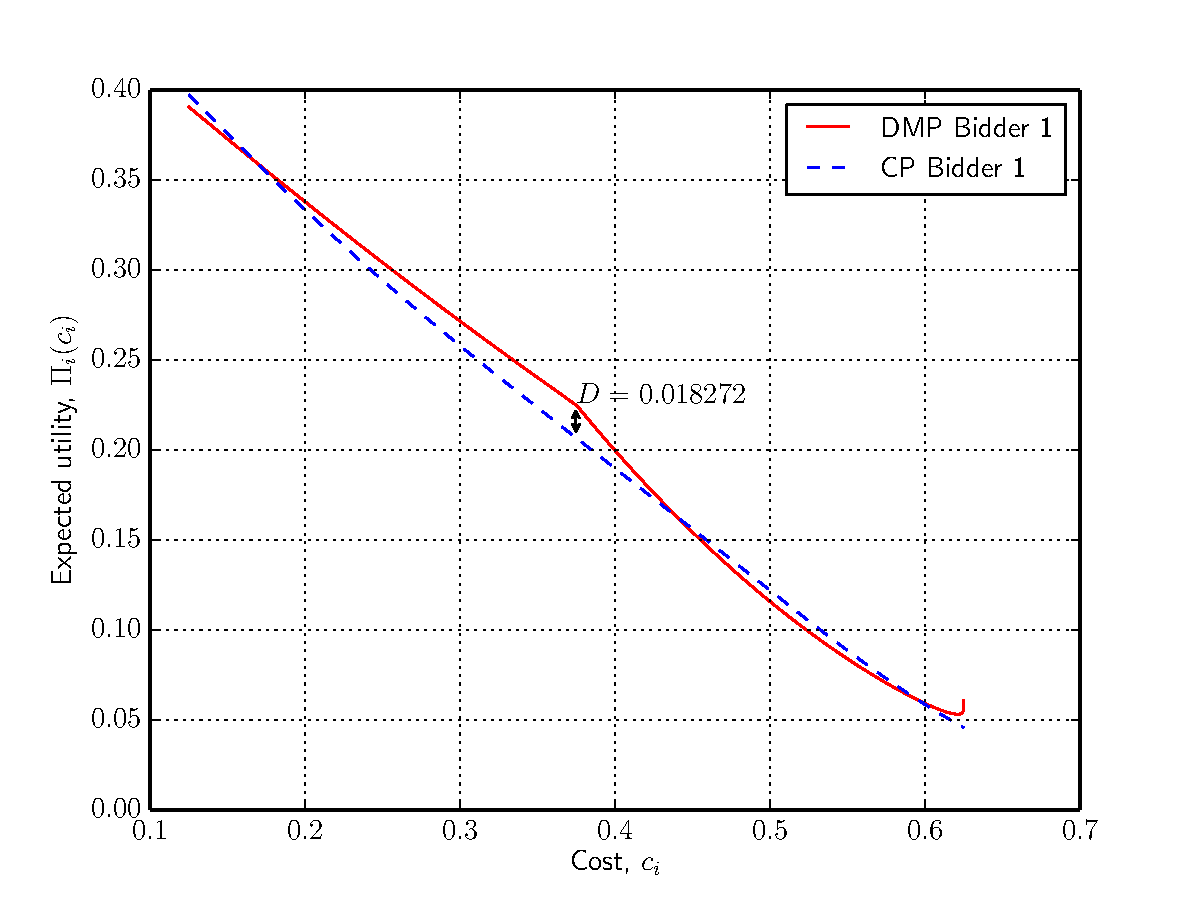
\includegraphics[width=\figsize]{Approximation/Figures/test_compare_bidder_1}
  \caption{FIX:ME}
  \label{fig:test_compare_bidder_1_approximation}
  \vspace{10mm}
  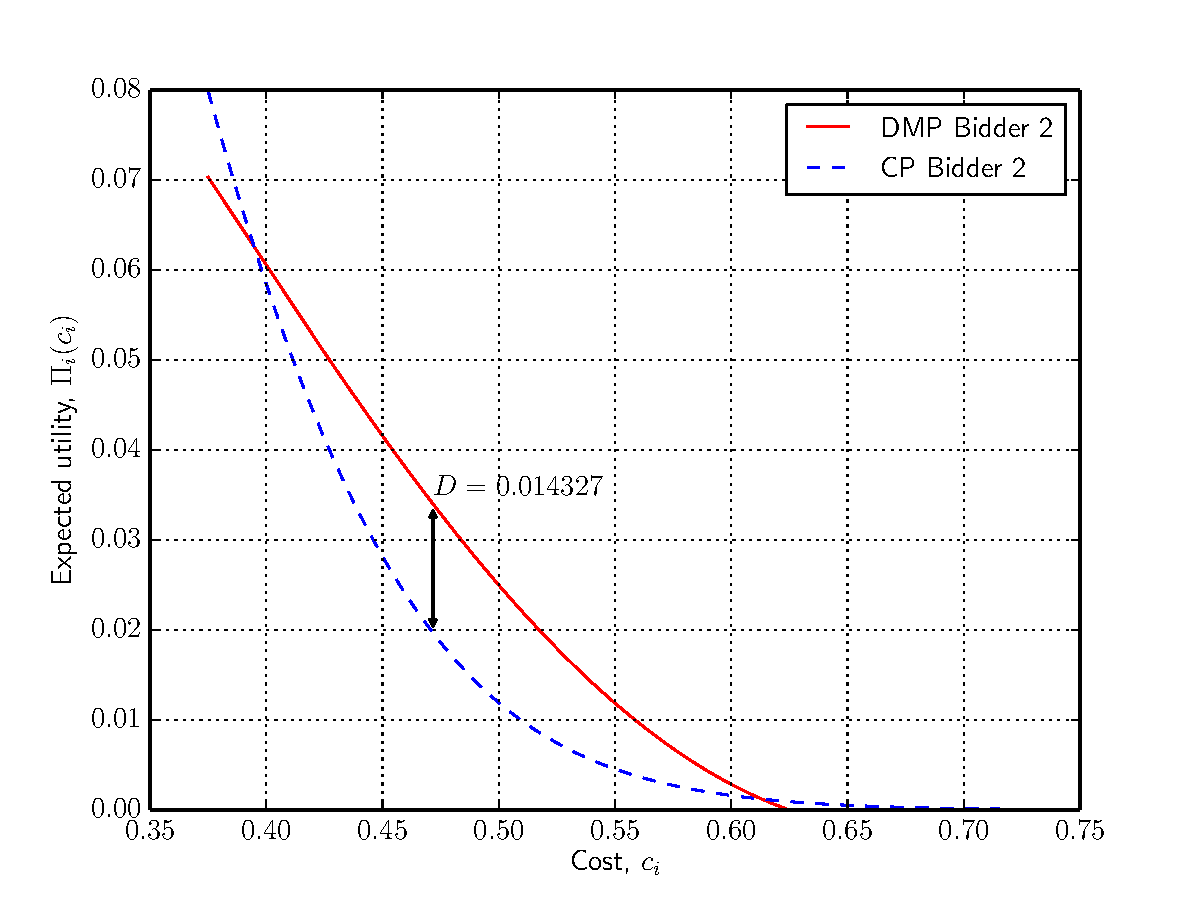
\includegraphics[width=\figsize]{Approximation/Figures/test_compare_bidder_2}
  \caption{FIX:ME}
  \label{fig:test_compare_bidder_2_approximation}
\end{figure}

\subsection{Methodology for Quantifying Accuracy of the Approximations} % (fold)
\label{sub:methodology_for_quantifying_accuracy_of_the_approximations_approximation}
There are two fundamental questions that need to be addressed when it comes to quantifying accuracy of the approximations. First, how can we compare the predictions (in terms of the equilibrium bidding strategies) produced by both auction types, and second, how such a comparison can be quantified to allow for a programmatic treatment of the problem (thus, removing the possibility of human error when visually comparing the results).

The most straightforward way of comparing the results generated by the approximation (CP) auction with those generated by the \emph{benchmark} (DMP) auction is to compare the expected profits (or utilities) for all bidders. We define the expected utility as
\begin{equation}
  \label{eq:expected_utility_approximation}
  \Pi_i(c_i) \equiv E[u_i(b,c)] = (b_i(c_i) - c_i)\cdot P\{\textrm{winning}\:\vert\: b_i(c_i)\}
\end{equation}
for all $i\in N$ where $b_i$ is the equilibrium bidding function.

It is important to note that expected utility is a function of cost. Thus, quantifying this comparison methodology is equivalent to measuring the difference (or distance/distortion) between two curves (two expected utility functions). This can be accomplished by adopting the Kolmogorov-Smirnov (K-S) statistic used in the statistical test, known as the Kolmogorov-Smirnov test, which is used to test whether a random sample comes from a reference probability distribution. Recall that the K-S statistic is defined by
\begin{equation*}
  D = \sup_x |G(x) - F(x)|
\end{equation*}
where $F(x)$ is the cdf of the reference probability distribution, $G(x)$ is the cdf of the random sample, and $x$ comes from the (common) domain of both functions. For the purpose of our comparison, we shall replace the cdf functions with expected utility functions for the corresponding bidders from both CP and DMP auctions, and the supremum with maximum since the expected utility functions are bounded; that is,
\begin{equation}
  \label{eq:k_s_statistic_approximation}
  \displaystyle D_i = \max_{c_i\in \mathscr{D}(\Pi_i^\textrm{DMP})} \left\vert\Pi_i^{\textrm{CP}}(c_i) - \Pi_i^{\textrm{DMP}}(c_i)\right\vert
\end{equation}
for all $i\in N$, where $\mathscr{D}$ denotes the domain of a function\footnote{The domain of the expected utility function for the CP auction will always contain (be the superset) of the corresponding domain for the DMP auction; that is, $\mathscr{D}(\Pi_i^\textrm{DMP})\subseteq\mathscr{D}(\Pi_i^\textrm{CP})$ (cf.~Equation~\eqref{eq:domain_common_priors_approximation})}.

Before presenting the results of approximations, consider the numerical example from the previous section. Figure~\ref{fig:test_compare_bidder_1_approximation} depicts the expected utility function for bidder 1 for both auctions, and similarly, Figure~\ref{fig:test_compare_bidder_2_approximation} for bidder 2. The K-S statistic for bidder 1 is equal to, $D_1=0.018272$, while bidder 2, $D_2=0.014327$. It is worth noting that the domains for the expected utility functions of each bidder in both auctions are equal. Furthermore, due to the nature of the FSM method, the generated solutions are described in terms of a discrete set points, and therefore, in the implementation of the described methodology, the generated set of expected utilities is interpolated before the K-S statistics are evaluated (see Appendix~\ref{cha:numerical_software} for more details on the implementation of the described methodology).

It is difficult to judge by the value of the K-S statistic how erroneous the approximation for each bidder is. For instance, in the numerical example discussed in the previous paragraph, even though the K-S statistics for each bidder are close in value, the statistic itself does not capture its value relative to the benchmark expected utility's range of values for the bidder; that is, the range of the expected utility for bidder 1 in the benchmark (DMP) auction goes from approximately $0.05$ to $0.38$ (cf.~Figure~\ref{fig:test_compare_bidder_1_approximation}), while for bidder 2 from $0$ to $0.07$ (cf.~Figure~\ref{fig:test_compare_bidder_2_approximation}). It is, therefore, clear that, even though the K-S statistics are close in value, the approximation error for bidder 1 is much smaller than for bidder 2. To account for this fact, we define the relative error of the approximation as
\begin{equation}
  \label{eq:relative_error_approximation}
  \epsilon_i = \frac{D_i}{|\bar{\pi}_i^{\textrm{DMP}} - \underline{\pi}_i^{\textrm{DMP}}|}
\end{equation}
for all $i\in N$, where $\Pi_i^{\textrm{DMP}}(c_i)\in [\underline{\pi}_i^{\textrm{DMP}}, \bar{\pi}_i^{\textrm{DMP}}]$ for all $c_i\in \mathscr{D}(\Pi_i^{\textrm{DMP}})$.

For the K-S statistic values in the numerical example discussed in the previous paragraph, the percentage relative error for bidder 1 is $\epsilon_1\approx 5.54\%$, while for bidder 2 $\epsilon_2\approx 20.47\%$. Clearly, $\epsilon_2 > \epsilon_1$, thus, capturing the error in approximation for both bidders accurately.
% subsection methodology (end)

\subsection{Results of Approximations} % (fold)
\label{sub:results_of_approximations_approximation}
This section presents the results of approximating the DMP auction with CP auction. We analyse the results for two scenarios: with $n=2$ and $n=3$ bidders respectively. In both scenarios, the reputation ratings are kept fixed for all the bidders as we slide across the price weight values: $w\in[0.5, 0.99]$ and $w\in[0.75,0.99]$ for the first and second bidding scenario respectively. Therefore, we concentrate on scenarios that do not require the use of the extended forward shooting method (cf.~assumptions of Section~\ref{sec:numerical_analysis_indirect}).

\subsubsection{$n=2$ Bidders} % (fold)
\label{ssub:n_2_bidders_approximation}
We consider 4 bidding scenarios where bidder 2 is always characterised by fixed reputation rating of $r_2=0.75$, while bidder 1's reputation rating assumes values $r_1\in\{0.15, 0.25, 0.5, 0.7\}$. Figure~\ref{fig:compare_2_bidders_approximation} depicts the results of the approximations.

\begin{figure}[p!]
  \vspace{0.5cm}
  \begin{subfigure}[b]{0.5\textwidth}
    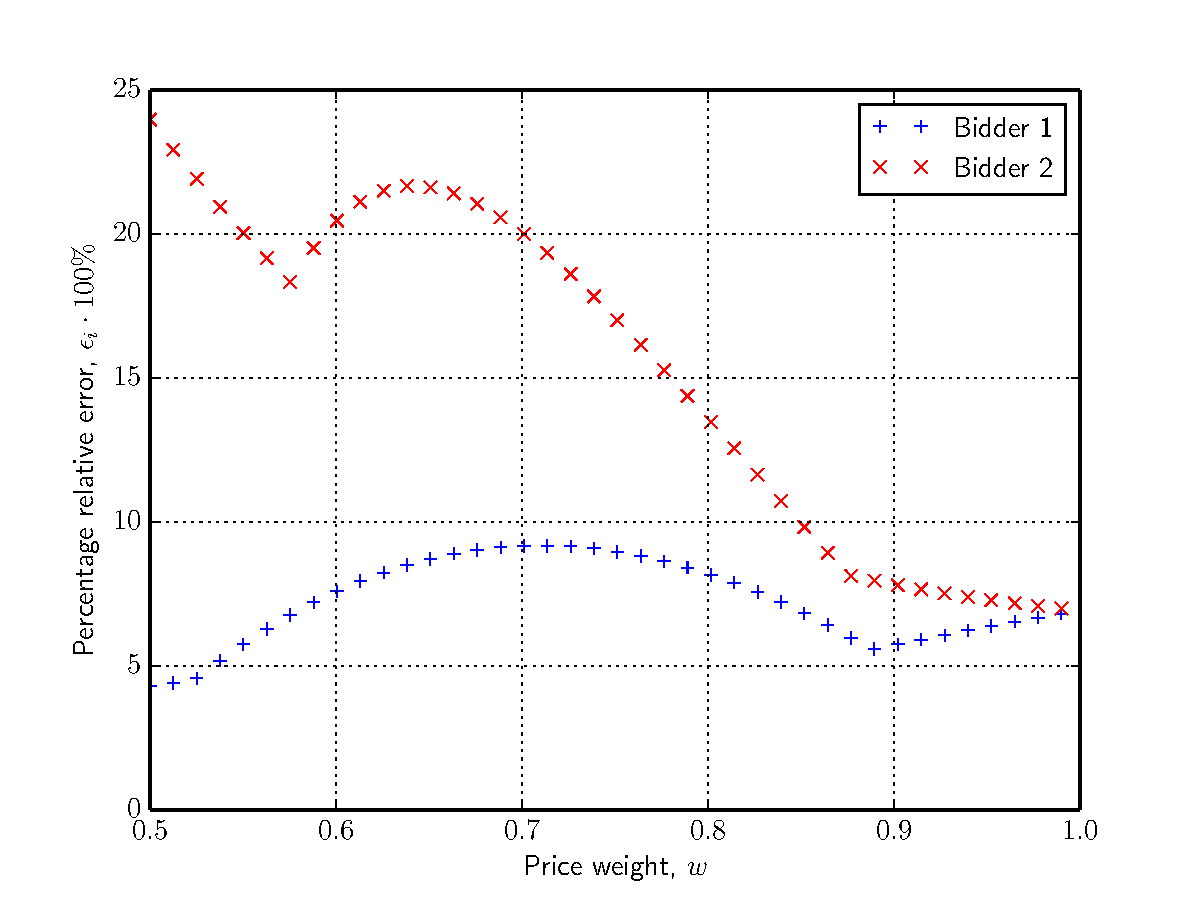
\includegraphics[width=3in]{Approximation/Figures/compare_2_bidders_015_075}
    \caption{FIX:ME $r_1=0.15$ and $r_2=0.75$}
    \label{fig:compare_2_bidders_015_075_approximation}
  \end{subfigure}
  \begin{subfigure}[b]{0.5\textwidth}
    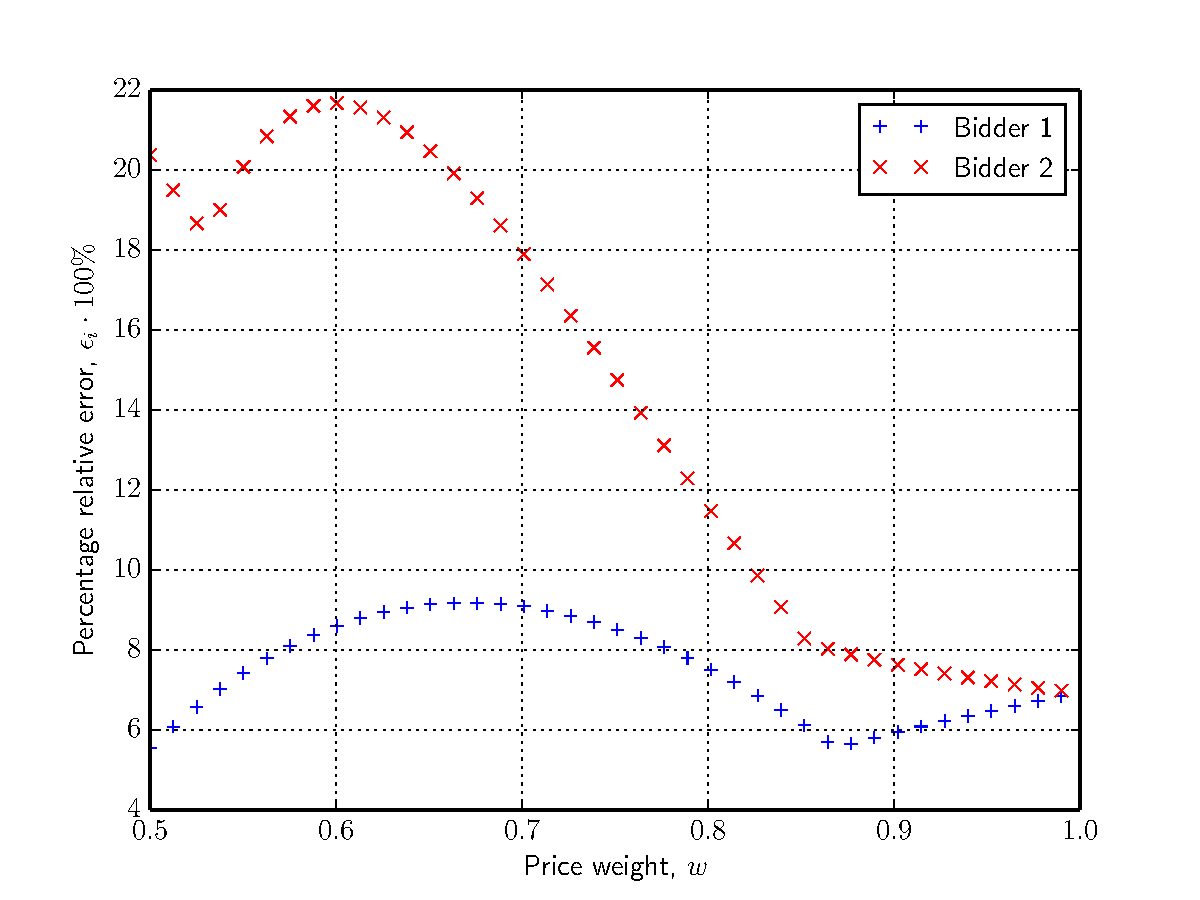
\includegraphics[width=3in]{Approximation/Figures/compare_2_bidders_025_075}
    \caption{FIX:ME $r_1=0.25$ and $r_2=0.75$}
    \label{fig:compare_2_bidders_025_075_approximation}
  \end{subfigure}
  \vspace{0.5cm}\\
  \begin{subfigure}[b]{0.5\textwidth}
    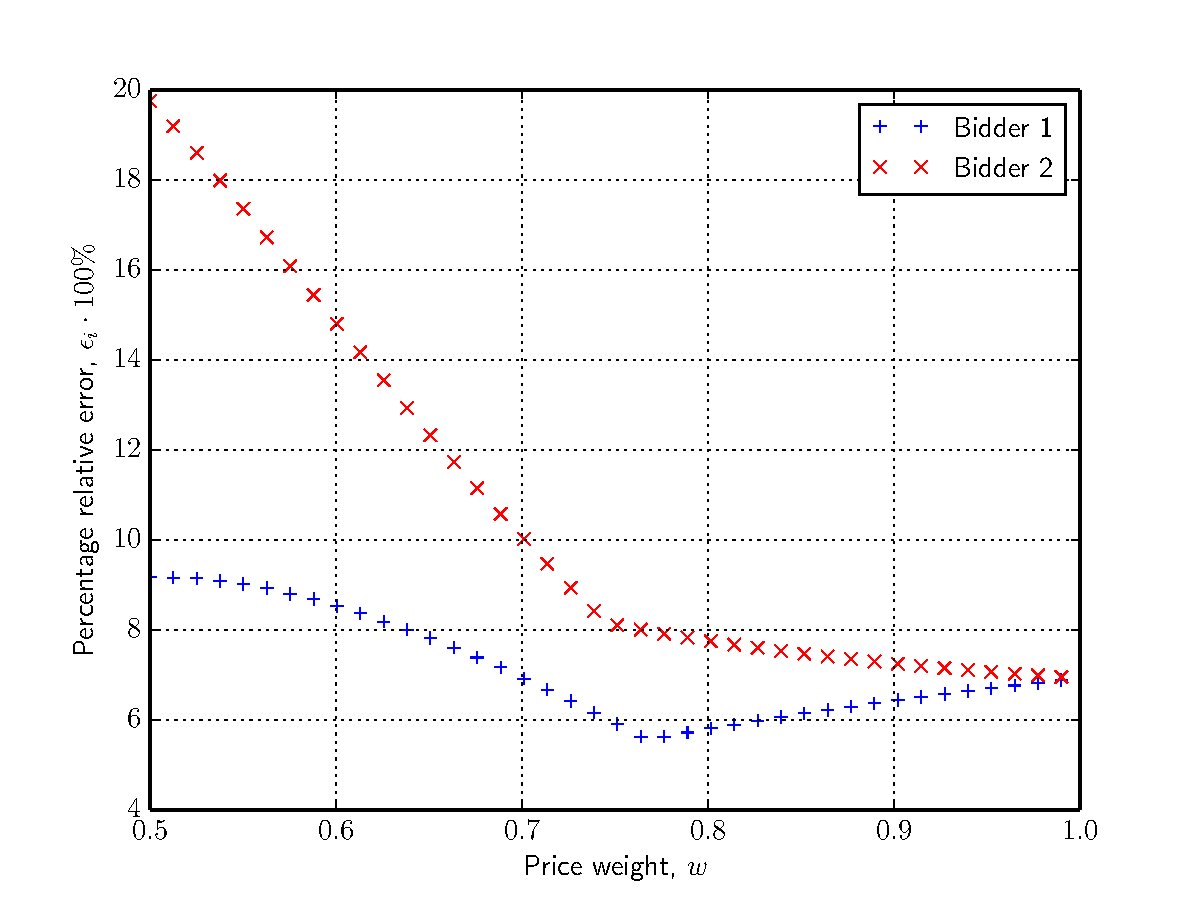
\includegraphics[width=3in]{Approximation/Figures/compare_2_bidders_050_075}
    \caption{FIX:ME $r_1=0.5$ and $r_2=0.75$}
    \label{fig:compare_2_bidders_050_075_approximation}
  \end{subfigure}
  \begin{subfigure}[b]{0.5\textwidth}
    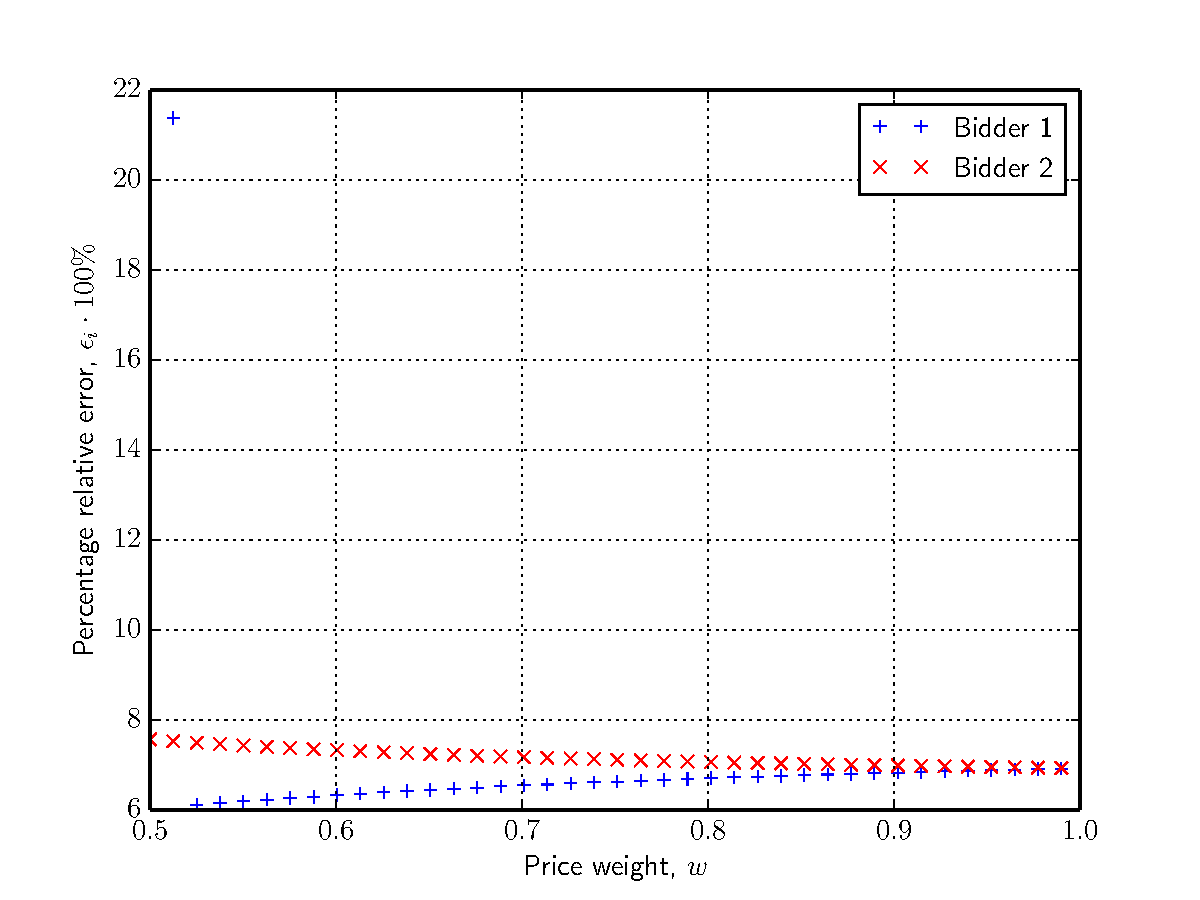
\includegraphics[width=3in]{Approximation/Figures/compare_2_bidders_070_075}
    \caption{FIX:ME $r_1=0.7$ and $r_2=0.75$}
    \label{fig:compare_2_bidders_070_075_approximation}
  \end{subfigure}
  \caption{FIX:ME}
  \label{fig:compare_2_bidders_approximation}
\end{figure}

In all cases, the percentage relative error is below $10\%$ for bidder 1, and below $25\%$ for bidder 2. Furthermore, for $r_1=0.7$ and $r_2=0.75$, the percentage relative error is below $8\%$ for both bidders. In fact, as the difference between $r_1$ and $r_2$ decreases, the shape of the percentage relative error curves, as a function of price weight, flattens out. The most likely explanation for this is the fact that as the difference between the reputation ratings decreases, the overlap between the supports for both bidders, $[\underline{c}_1, \bar{c}_1]$ and $[\underline{c}_2, \bar{c}_2]$, increases; thus, approaching the common priors setting closer and closer, to eventually reach a symmetric first-price sealed-bid auction for equal reputation ratings (cf.~Corollary~\ref{cor:special_case_r_i_r_j_direct}, Section~\ref{sub:special_case_r_i_r_j_direct}).

\begin{figure}[p!]
  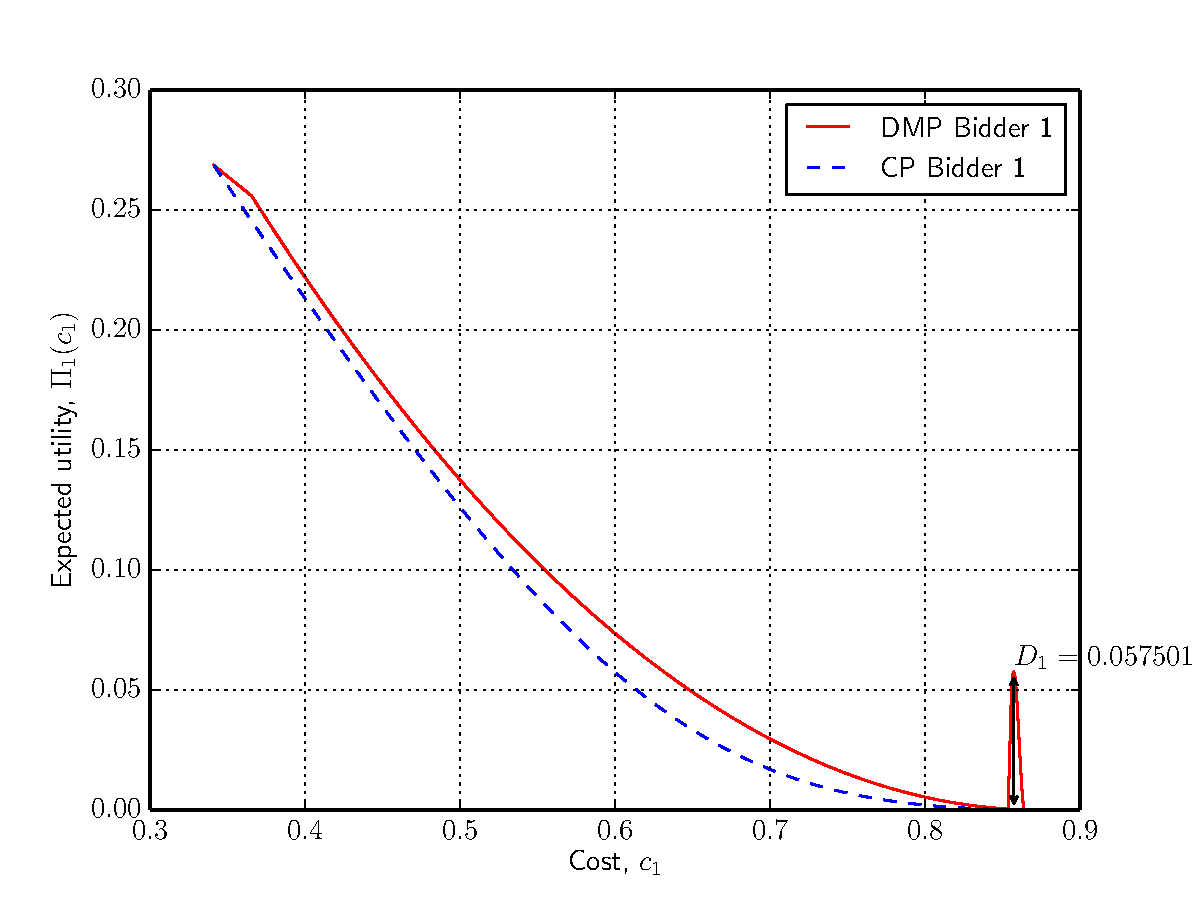
\includegraphics[width=\figsize]{Approximation/Figures/compare_2_bidders_070_075_outlier}
  \caption{FIX:ME}
  \label{fig:compare_2_bidders_070_075_outlier_approximation}
\end{figure}

It is worth noting that, in Figure~\ref{fig:compare_2_bidders_070_075_approximation}, there is an outlier at $w\approx 0.5125$ for bidder 1---their percentage relative error jumps from $6\%$ to almost $22\%$ to fall back again to $6\%$. This is due to the fact that the DMP version of the FSM method becomes numerically unstable near the upper bound on bids. This is a direct consequence of the problem not satisfying the Lipschitz condition for continuity (cf.~Section~\ref{sec:numerical_analysis_indirect}) for bid values approaching the upper bound on bids. As a result, the K-S statistic is incorrectly computed. Figure~\ref{fig:compare_2_bidders_070_075_outlier_approximation} depicts the expected utilities for bidder 1 in both DMP and CP auctions, and the associated, incorrectly computed, K-S statistic. Note that there is a considerable spike in the expected utility for the DMP bidder near the upper extremity of their support which is directly responsible for the outlier in Figure~\ref{fig:compare_2_bidders_070_075_approximation}.

All things considered, in the 2 bidders' case, approximating DMP auction with the CP auction does not yield small enough percentage relative error to consider it a viable alternative to solving the original, DMP auction. In fact, as presented next, the results are even less promising for 3 bidders.
% subsection n_2_bidders_approximation (end)

\subsubsection{$n=3$ Bidders} % (fold)
\label{ssub:n_3_bidders_approximation}
We consider 3 bidding scenarios where bidder 3 is always characterised by fixed reputation rating of $r_3=0.75$, while we vary reputation ratings of bidders 1 and 2: $r_1=0.25$ and $r_2=0.5$ (Figure~\ref{fig:compare_3_bidders_025_050_075_approximation}); $r_1=0.25$ and $r_2=0.7$ (Figure~\ref{fig:compare_3_bidders_025_070_075_approximation}); and $r_1=0.65$ and $r_2=0.75$ (Figure~\ref{fig:compare_3_bidders_065_070_075_approximation}). In what follows, the numerically derived equilibrium bidding strategies to the DMP auction are generated by both FSM and PPM methods.

\begin{figure}[p!]
  \begin{subfigure}[b]{0.5\textwidth}
    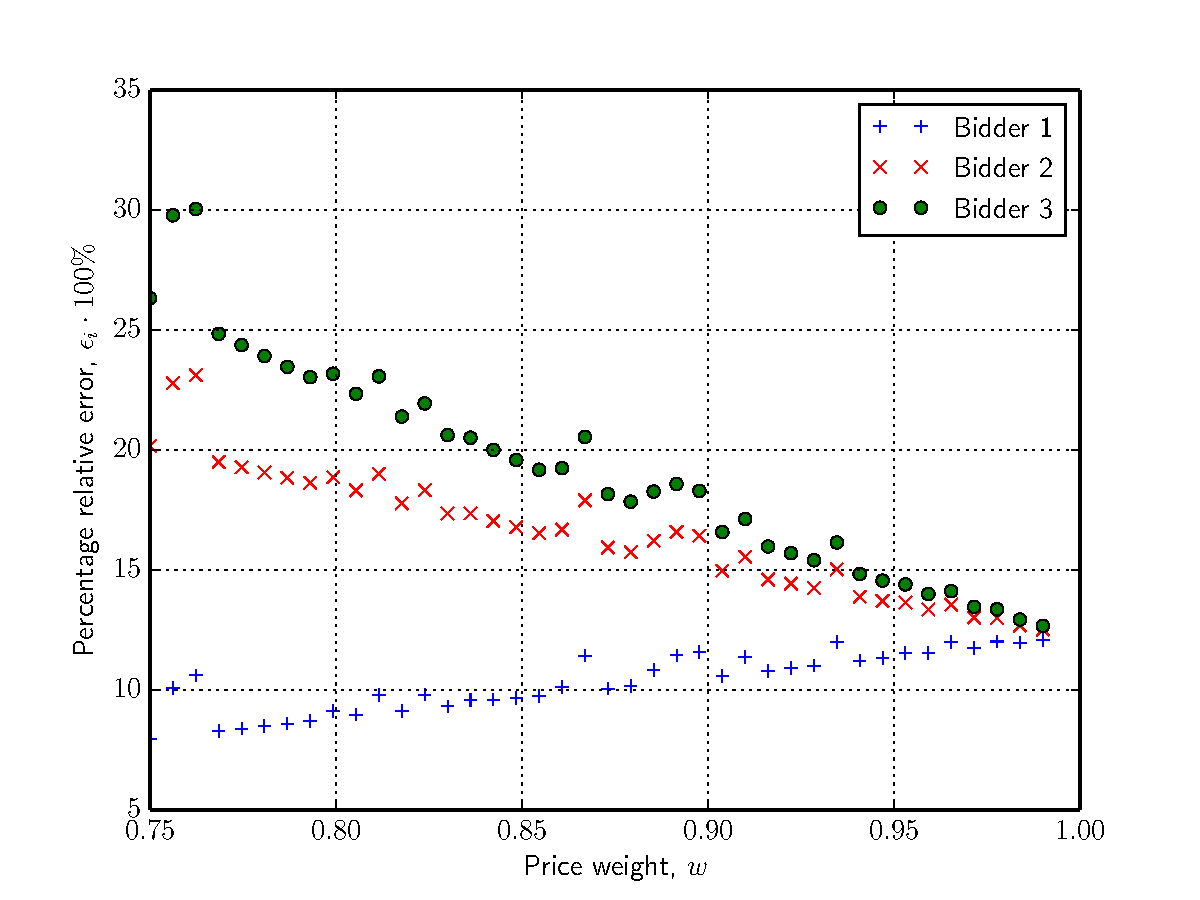
\includegraphics[width=3in]{Approximation/Figures/compare_3_bidders_025_050_075}
    \caption{FIX:ME $r_1=0.25$, $r_2=0.5$, and $r_3=0.75$ FSM}
    \label{fig:compare_3_bidders_025_050_075_fsm_approximation}
  \end{subfigure}
  \begin{subfigure}[b]{0.5\textwidth}
    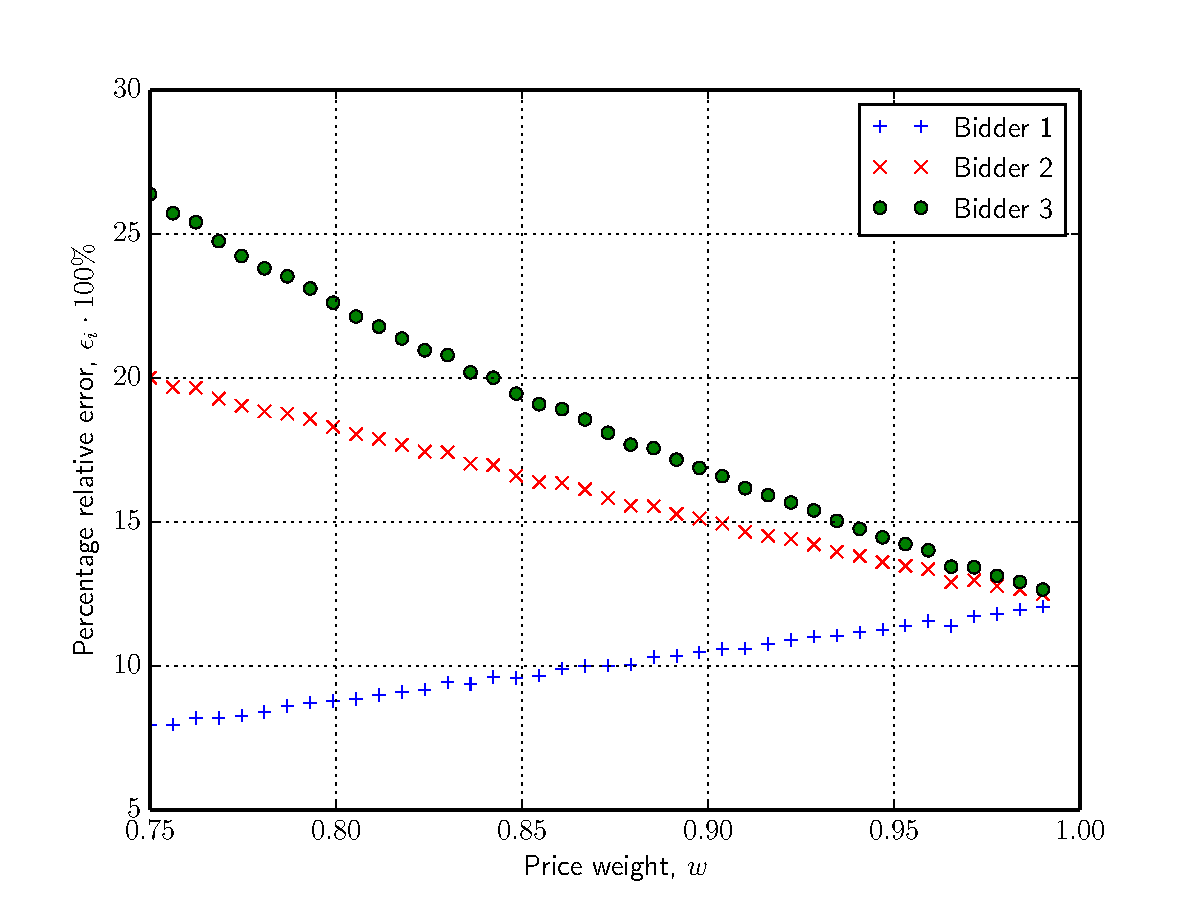
\includegraphics[width=3in]{Approximation/Figures/compare_3_bidders_025_050_075_ppm}
    \caption{FIX:ME $r_1=0.25$, $r_2=0.5$, and $r_3=0.75$ PPM}
    \label{fig:compare_3_bidders_025_050_075_ppm_approximation}
  \end{subfigure}
  \caption{FIX:ME}
  \label{fig:compare_3_bidders_025_050_075_approximation}
\end{figure}

\begin{figure}[p!]
  \setcounter{subfigure}{0}
  \begin{subfigure}[b]{0.5\textwidth}
    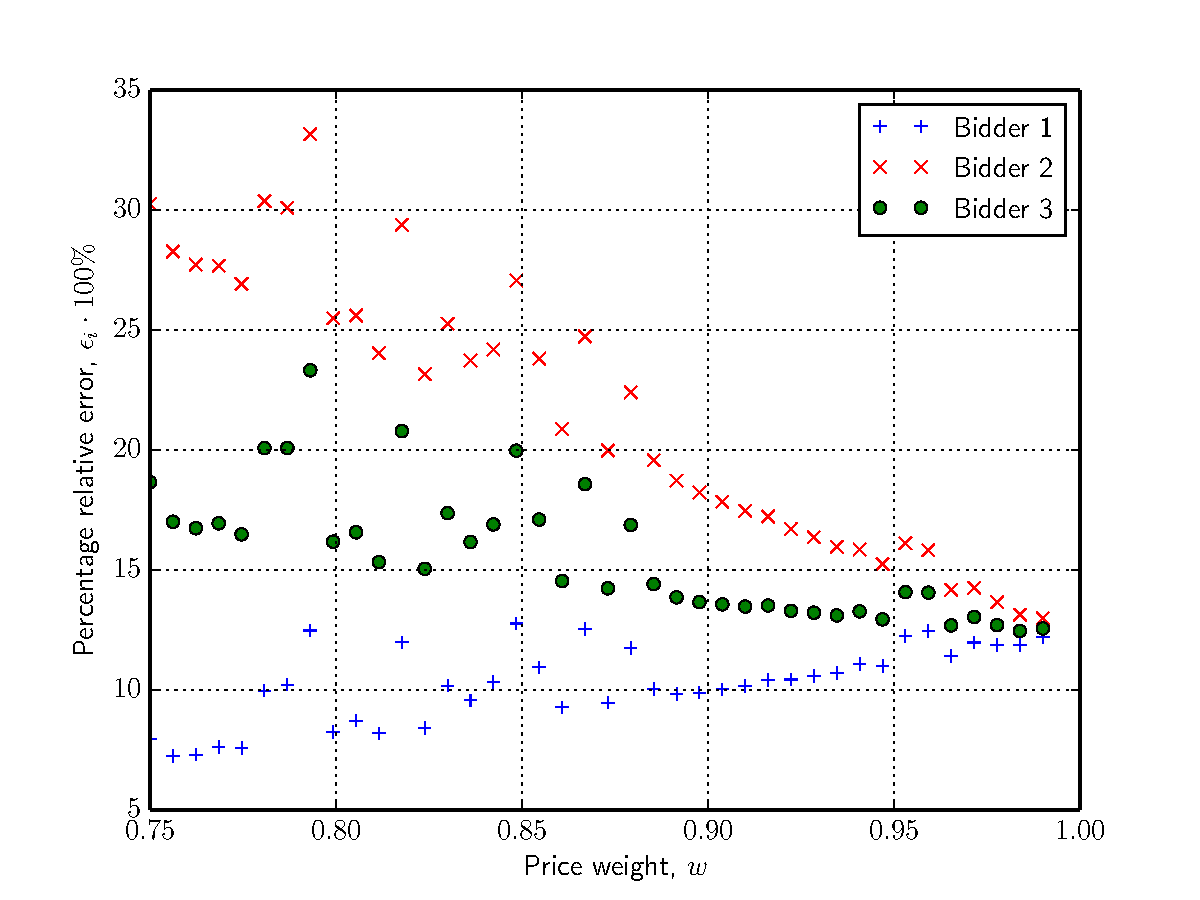
\includegraphics[width=3in]{Approximation/Figures/compare_3_bidders_025_070_075}
    \caption{FIX:ME $r_1=0.25$, $r_2=0.7$, and $r_3=0.75$ FSM}
    \label{fig:compare_3_bidders_025_070_075_fsm_approximation}
  \end{subfigure}
  \begin{subfigure}[b]{0.5\textwidth}
    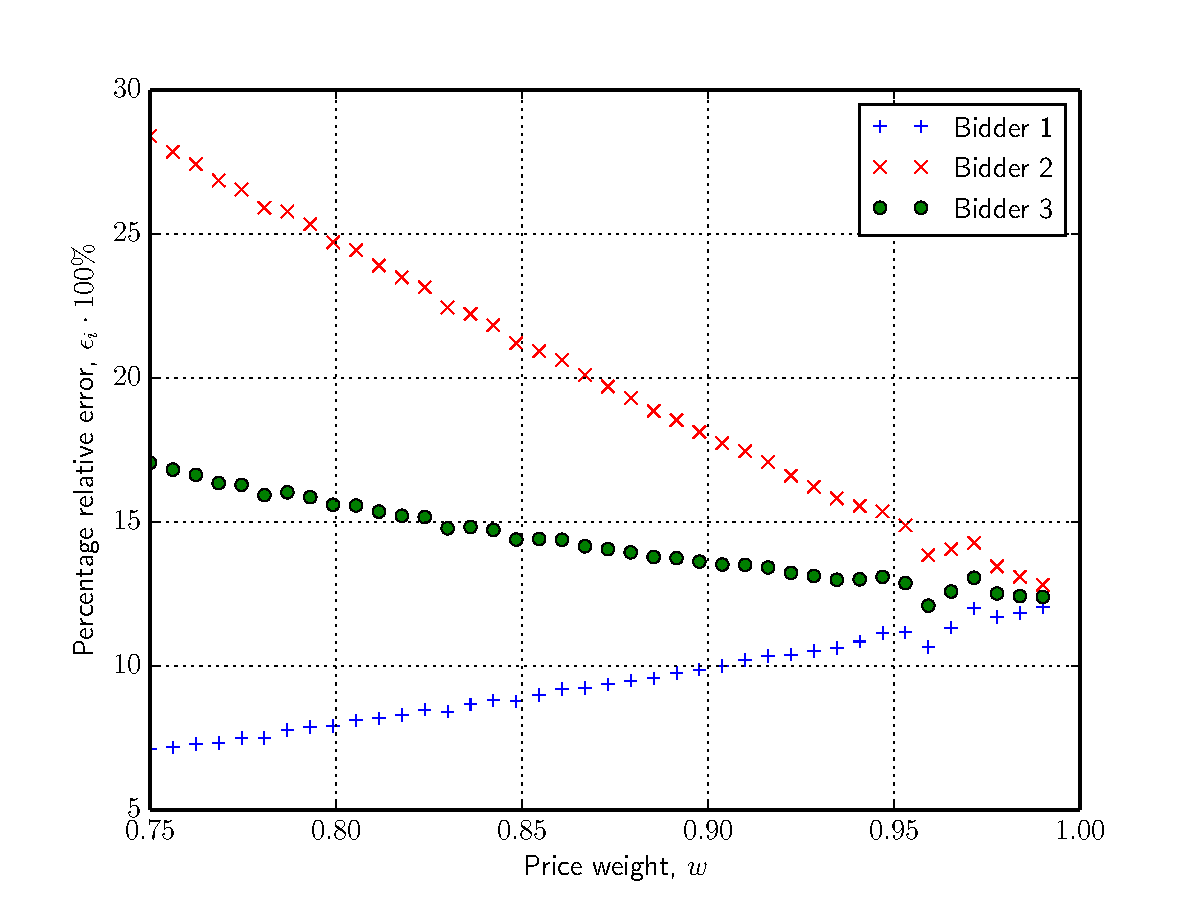
\includegraphics[width=3in]{Approximation/Figures/compare_3_bidders_025_070_075_ppm}
    \caption{FIX:ME $r_1=0.25$, $r_2=0.7$, and $r_3=0.75$ PPM}
    \label{fig:compare_3_bidders_025_070_075_ppm_approximation}
  \end{subfigure}
  \caption{FIX:ME}
  \label{fig:compare_3_bidders_025_070_075_approximation}
\end{figure}

\begin{figure}[p!]
  \begin{subfigure}[b]{0.5\textwidth}
    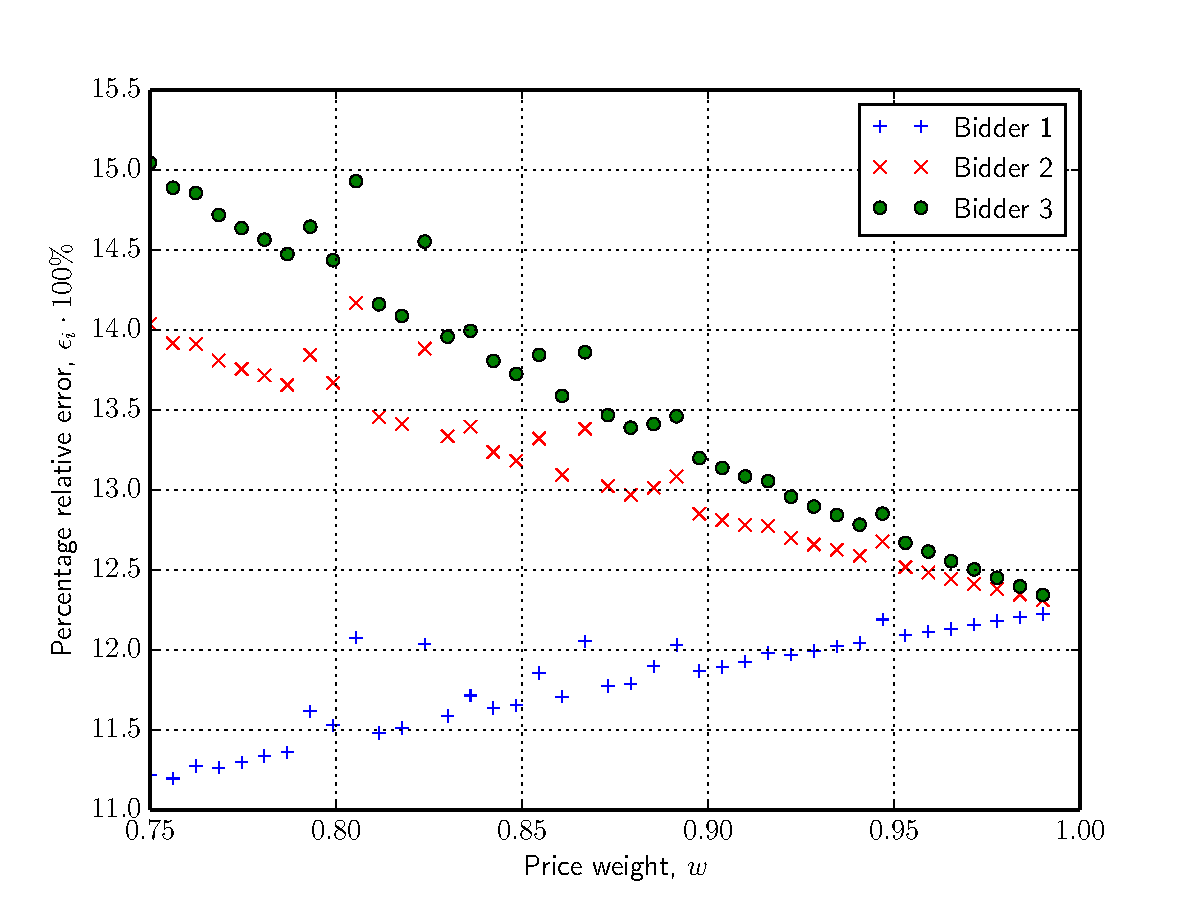
\includegraphics[width=3in]{Approximation/Figures/compare_3_bidders_065_070_075}
    \caption{FIX:ME $r_1=0.65$, $r_2=0.7$, and $r_3=0.75$ FSM}
    \label{fig:compare_3_bidders_065_070_075_fsm_approximation}
  \end{subfigure}
  \begin{subfigure}[b]{0.5\textwidth}
    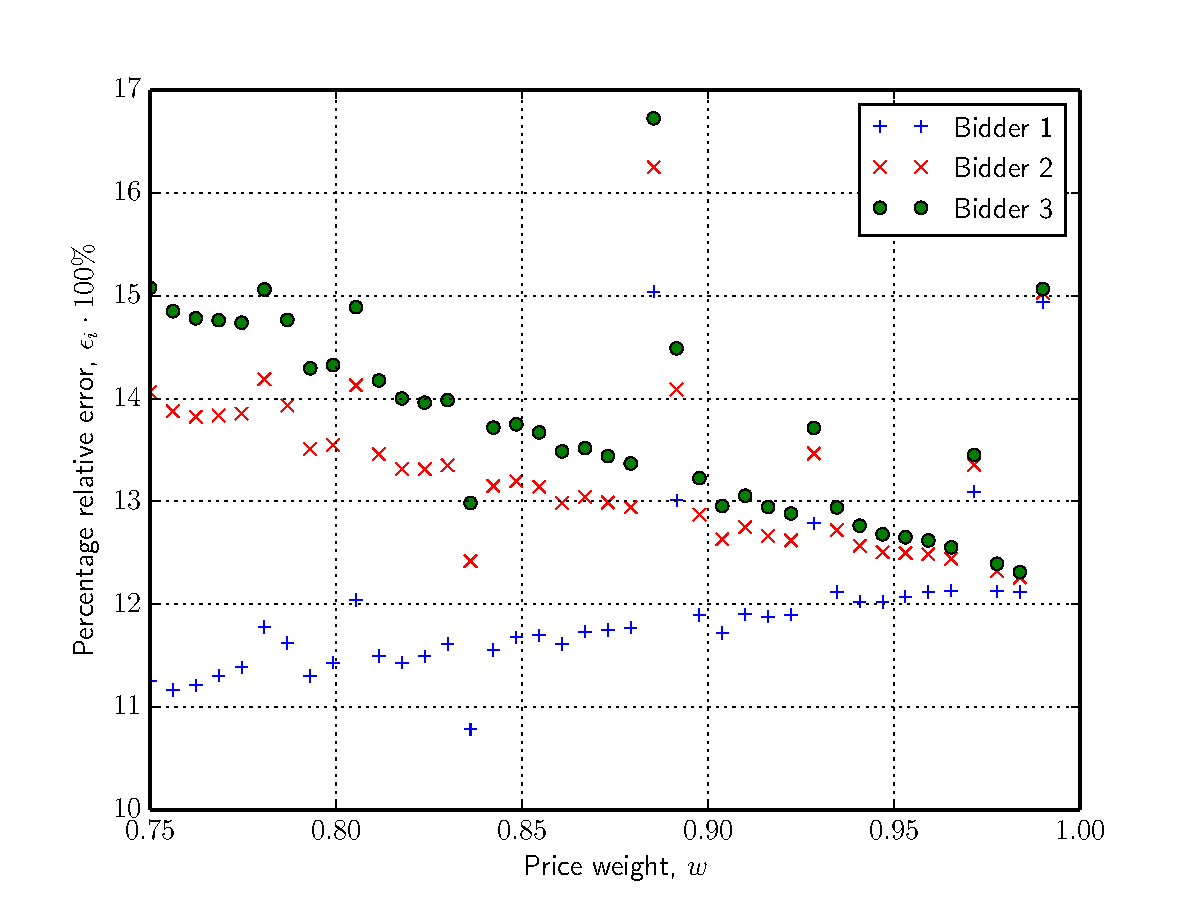
\includegraphics[width=3in]{Approximation/Figures/compare_3_bidders_065_070_075_ppm}
    \caption{FIX:ME $r_1=0.65$, $r_2=0.7$, and $r_3=0.75$ PPM}
    \label{fig:compare_3_bidders_065_070_075_ppm_approximation}
  \end{subfigure}
  \caption{FIX:ME}
  \label{fig:compare_3_bidders_065_070_075_approximation}
\end{figure}

Firstly, it should be noted that, for all bidding scenarios, the FSM method generates relatively noisy output, with the second bidding scenario being the noisiest (Figures~\ref{fig:compare_3_bidders_025_050_075_fsm_approximation} through to~\ref{fig:compare_3_bidders_065_070_075_fsm_approximation}). This is in contrast to very clean output generated by the PPM method to all bidding scenarios but the last one (Figures~\ref{fig:compare_3_bidders_025_050_075_ppm_approximation} through to~\ref{fig:compare_3_bidders_065_070_075_ppm_approximation}). The most likely explanation for the noisy output from the FSM method is due to, as discussed in Section~\ref{sub:approximation_results_indirect}, the FSM being inherently susceptible to the fact that the system of nonlinear ODEs does not satisfy the Lipschitz condition for continuity (which is especially true for $n>2$ bidders), and hence, the algorithm might not fully converge to the true solution of the system. This problem is eliminated entirely by the PPM method; still, however, in the last bidding scenario, the output is quite noisy.

Secondly, it is clear from the figures that, for all cases, the percentage relative error is below $13\%$ for bidder 1, and below $30\%$ for bidders 2 \& 3. As the price weight tends to 1 in all cases, the percentage relative error curves for all bidders converge to the same value of approximately $12\%$. All in all, it can be concluded that the percentage relative error is too high to consider the CP auction a viable alternative to solving the original, DMP auction.
% subsection n_3_bidders_approximation (end)
% subsection results (end)
% section network_selection_mechanism_cast_into_common_priors_setting (end)

\section{Summary} % (fold)
\label{sec:summary_approximation}

% section summary_approximation (end)

\section{Proofs} % (fold)
\label{sec:proofs_approximation}
\begin{proof}[Proof of Proposition~\ref{prop:characterization_of_the_equilibrium_in_common_priors_setting_approximation}]
The proposition is just a restatement of the Theorems C.1 Characterization of the Equilibria and U.1 Uniqueness of the Equilibrium in Lebrun~\cite{Lebrun2006}, and hence, we refer the Reader to that paper for proofs.
\end{proof}
% section proofs (end)
